\documentclass[10pt, aspectratio=169]{beamer}
\usepackage{caption}
\usepackage{subcaption}
\usetheme[progressbar=frametitle]{metropolis}
\usepackage{amsmath}
\usepackage{siunitx}
\usepackage{xcolor}
\usecolortheme{crane}
\definecolor{craneorange}{rgb}{0.53,0.66,0.42}
\usecolortheme{spruce}
\usepackage{hyperref}
\usepackage{multimedia}
\usepackage[percent]{overpic}
\usepackage[para]{footmisc}

\title{Computational study of far-field acoustic emission by collapsing bubbles}
\date{\today}
\author[shortname]{Magu Raam Prasaad R}
\institute[shortinst]{Indian Institute of Science, Bangalore}

\begin{document}

\begin{frame}
	\maketitle
\end{frame}

\begin{frame}{Computational approach}
	\begin{itemize}
		\item In this work we compute the far-field acoustic waves emitted from bubble collapse process using the Kirchhoff integral formulation.
	\end{itemize}

	\begin{figure}
		\centering
		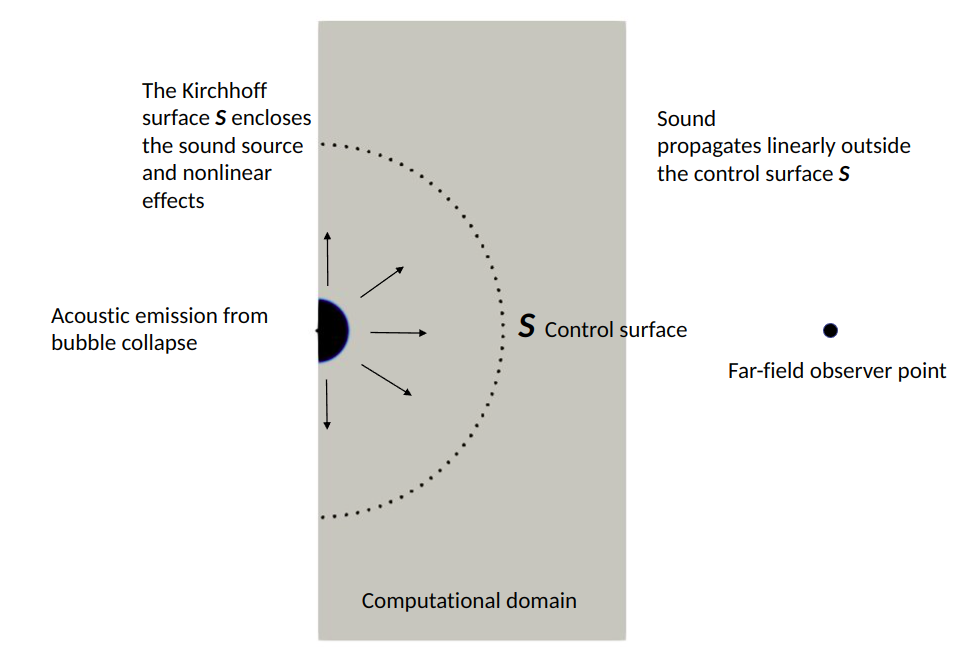
\includegraphics[scale=0.22]{images/schematic.png}
		\caption{Schematic of far-field acoustic data computed from CFD solver using the Kirchhoff integral method.}
	\end{figure}
\end{frame}

\begin{frame}{Kirchhoff integral formulation}
	\begin{itemize}
		\item The Kirchhoff integral equation for a stationary control surface is given by
		      \begin{equation}
			      \begin{split}
				      p'(\mathbf{x}, t) = \frac{1}{4\pi}\int_{S}\Big[  \frac{p'}{r'^{2}}\frac{\partial r'}{\partial n} - \frac{1}{r'}\frac{\partial p'}{\partial n} + \frac{1}{c r'}\frac{\partial r'}{\partial n}\frac{\partial p'}{\partial \tau} \Big]_{\tau} dS.
			      \end{split}
		      \end{equation}
		      $p'$ is the acoustic pressure satisfying the wave equation outside the control surface \textbf{S}, $c$ is the speed of sound at ambient conditions and $n$ is the normal.
		      The integrands are evaluated at the emission time $\tau = t - \mathbf{r'}/c$ and $\mathbf{r'}= |\mathbf{x} - \mathbf{y}|$ is the distance between observer and source.
		\item The $p'$, ${\partial p'}/{\partial t}$ and ${\partial p'}/{\partial n}$ are computed from flow solver.
	\end{itemize}
\end{frame}
\begin{frame}{Interpolation of pressure data}
	\begin{columns}
		\column{0.4\textwidth}
		\begin{figure}
			\centering
			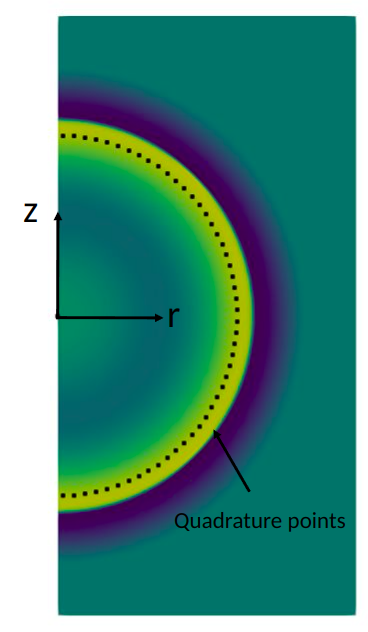
\includegraphics[scale=0.21]{images/arc.png}
			\caption{The fourth-order WENO polynomial is used to interpolate the data at quadrature points and the four-point Lagrange polynomial is used to interpolate the data at the emission time.}
		\end{figure}
		\column{0.4\textwidth}
		\begin{figure}
			\centering
			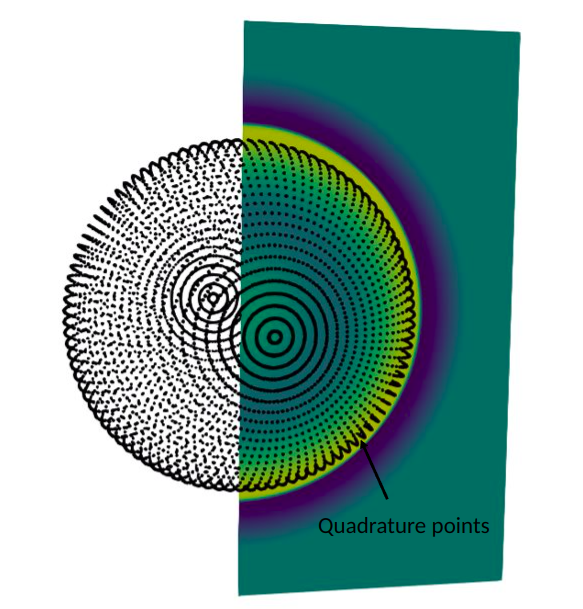
\includegraphics[scale=0.21]{images/sphere.png}
			\caption{Using the axi-symmetry, the pressure data is copied along the azimuthal direction. We can use the Kirchhoff intergal on a spherical surface to compute the far-field pressure.}
		\end{figure}
	\end{columns}
\end{frame}

\begin{frame}{Kirchhoff integral on a sphere}
	\begin{itemize}
		\item We compute the Kirchhoff integral on a spherical surface 
		\begin{equation}
			\begin{split}
				p'(r, \theta, \phi,t) =  \frac{1}{4\pi}\int_{0}^{2\pi}\int_{0}^{\pi}\Big[  \frac{p'}{r'^{2}}&\frac{\partial r'}{\partial n} - \frac{1}{r'}\frac{\partial p'}{\partial n} + \frac{1}{c r'}\frac{\partial r'}{\partial n}\frac{\partial p'}{\partial \tau} \Big]_{\tau} R^2\sin\theta d\theta d \phi  
			\end{split} 
		\end{equation}
		\item The above integral is numerically computed using the mid-point rule 
		\begin{equation}
			\begin{split}
				p'(r, \theta, \phi,t) =  \frac{1}{4\pi} \sum_{i}^{N_{\theta}}\sum_{j}^{N_{\phi}}  \Big[  \frac{p'}{r'^{2}}&\frac{\partial r'}{\partial n} - \frac{1}{r'}\frac{\partial p'}{\partial n} + \frac{1}{c r'}\frac{\partial r'}{\partial n}\frac{\partial p'}{\partial \tau} \Big]_{\tau} R^2\sin\theta \Big|_{i, j} \Delta \theta \Delta \phi  
			\end{split} 
		\end{equation}
	\end{itemize}
\end{frame}

\begin{frame}{Results: Computation of acoustic waves from Rayleigh collapse}
							
	\begin{columns}
		\begin{column}{0.45\textwidth}
			\begin{itemize}
				\item air bubble in water
				\item Axi-symmetric domain $\Omega = [-10R,10R]\times[0,10R]$
				\item Radius of the bubble $R = 38$
				\item Discretization $500\times 250$ cells
				\item Boundary conditions:
				      \begin{itemize}
				      	\item top, bottom, left and right boundary $-$ transmissive 
				      \end{itemize}
			\end{itemize}
		\end{column}
																																			
		\begin{column}{0.46\textwidth}
			\begin{figure}
				\centering
				\begin{overpic}[scale=0.28,unit=1mm]{images/initial_condition.png}
					\put (10,81) {$\displaystyle \textcolor{white}{Water}$}
					\put (10,74) {\textcolor{white}{$\displaystyle \rho = 10^{3}$}}
					\put (10,67) {\textcolor{white}{$\displaystyle p = 1.0$ }}
					\put (10,60) {\textcolor{white}{$\displaystyle \gamma = 4.4$ }}															
					\put (10,53) {\textcolor{white}{$\displaystyle P_{\infty} = 6000$ }}															
					

					\put (5,37) {$\displaystyle \textcolor{white}{Air}$}
					\put (5,30) {\textcolor{white}{$\displaystyle \rho = 1.0 $}}
					\put (5,23) {\textcolor{white}{$\displaystyle p = 0.1$}}
					\put (5,16) {\textcolor{white}{$\displaystyle \gamma = 1.4$ }}
					\put (5,9) {\textcolor{white}{$\displaystyle  P_{\infty} = 0$ }}


				\end{overpic}
				\caption{Initial condition}
			\end{figure}
		\end{column}
														
	\end{columns}
\end{frame}

\begin{frame}{Results: Computation of acoustic waves from Rayleigh collapse}
							
	\begin{columns}
		\begin{column}{0.45\textwidth}
			\begin{itemize}
				\item The radius of the spherical Kirchhoff surface is $6R$
				\item The far-field observer point is at $(0, 9R)$ 
				\item The number of quadrature points $N_{\theta} = 500$ and $N_{\phi} = 1000$
				\item The speed of sound in the far-field acoustic medium is given by $\sqrt{\gamma(P + P_{\infty})/\rho} = 66.5$	
			\end{itemize}
		\end{column}
																																			
		\begin{column}{0.46\textwidth}
			\begin{figure}
				\centering
				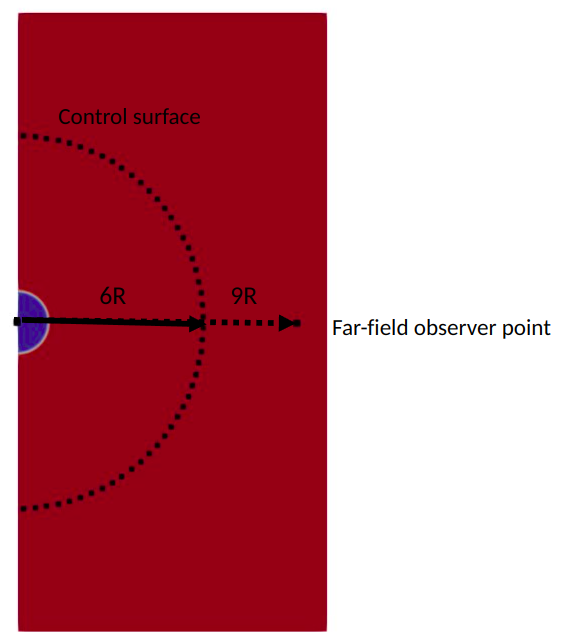
\includegraphics[scale=0.28]{images/schematic3.png}
				\caption{Location of control surface and observer point}
			\end{figure}
		\end{column}
														
	\end{columns}
\end{frame}
\begin{frame}{Results: Computation of acoustic waves from Rayleigh collapse}
	\begin{columns}
		\begin{column}{0.45\textwidth}
			\begin{figure}
				\centering
				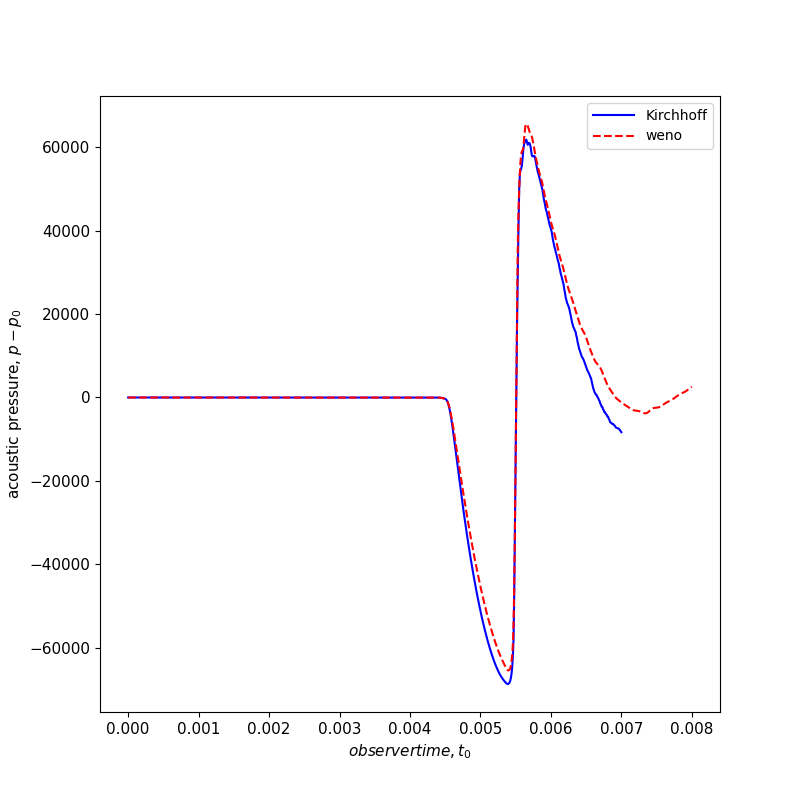
\includegraphics[scale=0.3]{images/structured_pressure.png}
				\caption{Comparison of acoustic pressure at observer point from flow solver and Kirchhoff solver.}
			\end{figure}
		\end{column}
		\begin{column}{0.55\textwidth}
			\begin{tabular}{ |c|c| } 
				\hline
				observer time, $t_{0}$   & relative error, $|\frac{p'_{kirchhoff} - p'_{weno}}{p'_{weno}}|$  \\ 
				\hline
				5.00e-03  & 1.29e-01 \\
				6.00e-03  & 3.99e-02 \\
				7.00e-03 &  6.03e+00 \\
			
				\hline
			\end{tabular}
		\end{column}
	\end{columns}	
\end{frame}
\begin{frame}{Conclusion}
	\begin{itemize}
		\item In this work we have compared the far-field acoustic pressure computed from the flow solver and the Kirchhoff solver for the collapse of a single bubble.   
		\item At observer point $(0, 9R)$ and the observer time,  $t_0 = .007$ the relative error is $6.03$.
		\item This shows the Kirchhoff solver does not predict the far-field pressure accurately. This might be due to the boundary condition as the observer point is located near the domain boundary.  
	\end{itemize}
\end{frame}
\begin{frame}[standout]
	Thank you!
\end{frame}
\end{document}

